\section{Reconhecimento de tokens}

\begin{frame}[fragile]{Fragmento de gramática que será utilizada nos exemplos}

\[
    \begin{array}{lcl}
        cmd & \to & \mathbf{if}\ expr\ \mathbf{then}\ cmd \\
            & |\ & \mathbf{if}\ expr\ \mathbf{then}\ cmd\ \mathbf{else}\ cmd \\
            & |\ & \code{apl}{∊} \\
        \\
        expr & \to & termo\ \mathbf{relop}\ termo \\
            & |\ & termo \\
        \\
        termo & \to&  \mathbf{id} \\
            & |\ & \mathbf{num} 
    \end{array}
\]

\end{frame}

\begin{frame}[fragile]{Definições regulares dos tokens}

\[
    \begin{array}{rcl}
        \mathbf{if} & \to & \texttt{if} \\ 
        \mathbf{then} & \to & \texttt{then} \\ 
        \mathbf{else} & \to & \texttt{else} \\ 
        \mathbf{relop} & \to & \texttt{< | <= | = | <> | > | >=} \\ 
        \mathbf{letra} & \to & \texttt{A | B | ... | Z | a | b | ... | z} \\
        \mathbf{dígito} & \to & \texttt{0 | 1 | 2 | ... | 9} \\
        \mathbf{id} & \to & \mathbf{letra}\ (\mathbf{letra}\ |\ \mathbf{dígito})^* \\
        \mathbf{num} & \to & \mathbf{dígito}^+ (\texttt{.}\ \mathbf{dígito}^+)?(\texttt{E}(\texttt{+|-})?\ \mathbf{dígito}^+)?\\
    \end{array}
\]

\end{frame}

\begin{frame}[fragile]{Tratamento de espaços em branco}

    \begin{itemize}
        \item Assuma que os lexemas sejam separados por espaços em brancos
       %\pause

        \item São considerados espaços em branco: sequências de espaços em branco, tabulações e quebras de linha
       %\pause

        \item O analisador léxico deve ignorar os espaços em branco
       %\pause

        \item A definição regular $\mathbf{ws}$ identifica os espaços em branco:
        \[
            \begin{array}{rcl}
                \mathbf{delim} & \to & \mathbf{branco}\ |\ \mathbf{tabulação}\ |\ \mathbf{quebra de linha}\\
                \mathbf{ws} & \to & \mathbf{delim}^+
            \end{array}
        \]
       %\pause

        \item Se o analisador léxico identificar o padrão $\mathbf{ws}$, ele não irá gerar um token
    \end{itemize}

\end{frame}

\begin{frame}[fragile]{Especificação dos tokens}

    \begin{table}
        \centering

    \begin{tabularx}{0.7\textwidth}{ccX}
        \toprule
        \textbf{Expressão regular} & \textbf{Token} & \textbf{Valor do atributo} \\
        \midrule
        $\mathbf{ws}$ & - & - \\
        \texttt{if} & $\mathbf{if}$ & - \\
        \texttt{then} & $\mathbf{then}$ & - \\
        \texttt{else} & $\mathbf{else}$ & - \\
        \texttt{id} & $\mathbf{id}$ & Lexema \\
        \texttt{num} & $\mathbf{num}$ & Valor numérico do lexema \\
        \texttt{<} & $\mathbf{relop}$ & \texttt{LT} \\
        \texttt{<=} & $\mathbf{relop}$ & \texttt{LE} \\
        \texttt{=} & $\mathbf{relop}$ & \texttt{EQ} \\
        \texttt{<>} & $\mathbf{relop}$ & \texttt{NE} \\
        \texttt{>} & $\mathbf{relop}$ & \texttt{GT} \\
        \texttt{>=} & $\mathbf{relop}$ & \texttt{GE} \\
        \bottomrule
    \end{tabularx}
    \end{table}

\end{frame}

\begin{frame}[fragile]{Diagramas de transição}

    \begin{itemize}
        \item Um diagrama de transição é um fluxograma estilizado que delineia as ações a serem tomadas pelo analisador léxico a cada requisição de novo token
            por parte do \textit{parser}
       %\pause

        \item Os estados são representados por círculos rotulados e identificam posições do diagrama 
       %\pause

        \item As transições são representadas por arestas direcionadas, rotuladas por um caractere
       %\pause

        \item Uma transição do estado \texttt{X} para o estado \texttt{Y} cujo rótulo é o caractere $c$ indica que, se a execução está no estado \texttt{X} e
            o próximo caractere lido é $c$, então a execução deve consumir $c$ e seguir para o estado \texttt{Y}
       %\pause

        \item Um diagrama de transição é determinístico se todas as transições que partem de um estado são rotuladas por caracteres distintos
    \end{itemize}

\end{frame}

\begin{frame}[fragile]{Estados e ações}

    \begin{itemize}
        \item Um estado deve ser rotulado como estado de partida, o qual marca o início da execução
       %\pause

        \item Se os rótulos dos estados são numéricos, a convenção é que o estado inicial seja o de número zero (ou um)
       %\pause

        \item Alguns estados podem ter ações associadas, as quais são executadas quando a execução atinge tal estado
       %\pause

        \item Executada a ação, se existir, deve ser lido o próximo caractere $c$ da entrada: se existir uma transição rotulada por $c$, a execução segue
            para o novo estado, indicado pela aresta; caso contrário, deve ser sinalizado um erro
       %\pause

        \item Os estados de aceitação, que indicam que um token foi reconhecido, são marcados com um círculo duplo
    \end{itemize}

\end{frame}

\begin{frame}[fragile]{Retrações e erros léxicos}

    \begin{itemize}
        \item Um estado de aceitação que demande o retorno do último caractere lido para o buffer de entrada é marcado um símbolo \texttt{*}
       %\pause

        \item Isto ocorre, por exemplo, em casos em que um token é finalizado por um espaço ou por um caractere que inicia um novo token
       %\pause

        \item Um analisador léxico pode ter vários diagramas de transição
       %\pause

        \item Se acontecer um erro no fluxo de execução de um diagrama, o ponteiro de leitura deve ser reposicionado ao ponto que estava no estado de partida
            e um novo diagrama deve ser seguido
       %\pause

        \item Se ocorrem erros em todos os diagramas, então há um erro léxico no programa fonte 
    \end{itemize}

\end{frame}

\begin{frame}[fragile]{Diagrama de transição para operadores relacionais}

    \begin{figure}
        \centering

        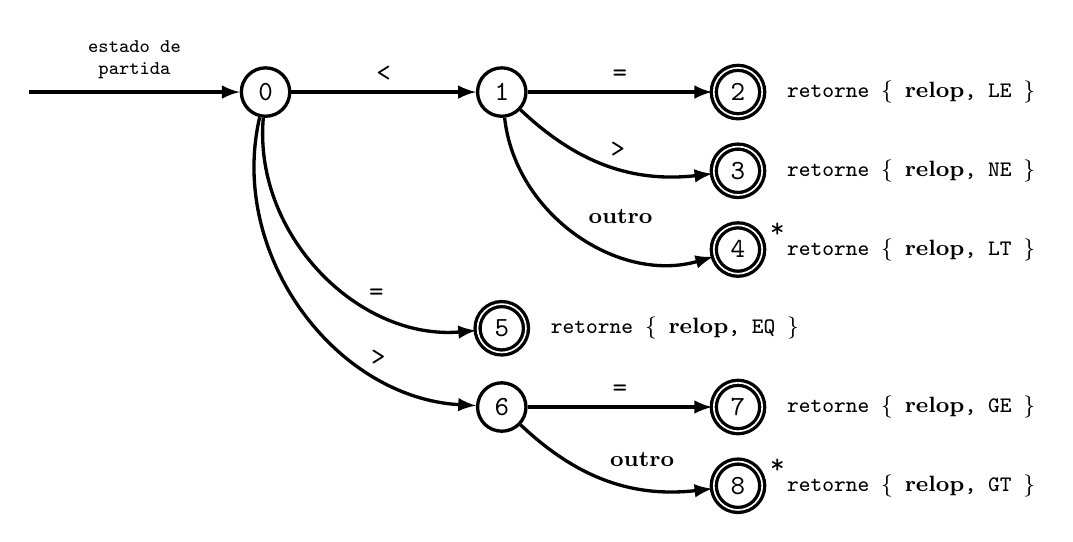
\begin{tikzpicture} 
            \coordinate (X) at (0, 6);

            \node[draw,circle,very thick] (A0) at (3, 6) { \texttt{0} };
            \node[draw,circle,very thick] (A1) at (6, 6) { \texttt{1} };
            \node[draw,circle,double,very thick] (A2) at (9, 6) { \texttt{2} };
            \node[draw,circle,double,very thick] (A3) at (9, 5) { \texttt{3} };
            \node[draw,circle,double,very thick] (A4) at (9, 4) { \texttt{4} };
            \node[draw,circle,double,very thick] (A5) at (6, 3) { \texttt{5} };
            \node[draw,circle,very thick] (A6) at (6, 2) { \texttt{6} };
            \node[draw,circle,double,very thick] (A7) at (9, 2) { \texttt{7} };
            \node[draw,circle,double,very thick] (A8) at (9, 1) { \texttt{8} };

            \node at (9.5, 4.25) { \texttt{*} };
            \node at (9.5, 1.25) { \texttt{*} };

            \node[anchor=west] at (9.5, 6) { \footnotesize \texttt{retorne \{ $\mathbf{relop}$, LE\ \}} };
            \node[anchor=west] at (9.5, 5) { \footnotesize \texttt{retorne \{ $\mathbf{relop}$, NE\ \}} };
            \node[anchor=west] at (9.5, 4) { \footnotesize \texttt{retorne \{ $\mathbf{relop}$, LT\ \}} };
            \node[anchor=west] at (6.5, 3) { \footnotesize \texttt{retorne \{ $\mathbf{relop}$, EQ\ \}} };
            \node[anchor=west] at (9.5, 2) { \footnotesize \texttt{retorne \{ $\mathbf{relop}$, GE\ \}} };
            \node[anchor=west] at (9.5, 1) { \footnotesize \texttt{retorne \{ $\mathbf{relop}$, GT\ \}} };

            \draw[very thick,-latex] (X) to node[above] { \scriptsize \texttt{\begin{tabular}{c}estado de\\ partida\end{tabular}} } (A0);
            \draw[very thick,-latex] (A0) to node[above] { \texttt{<} } (A1);
            \draw[very thick,-latex] (A1) to node[above] { \texttt{=} } (A2);
            \draw[very thick,-latex] (A1) [bend right=25] to node[above,pos=0.55] { \texttt{>} } (A3);
            \draw[very thick,-latex] (A1) [bend right=50] to node[above right,pos=0.5] { \footnotesize $\mathbf{outro}$ } (A4);
            \draw[very thick,-latex] (A0) [bend right=50] to node[above, pos=0.7] { \texttt{=} } (A5);
            \draw[very thick,-latex] (A0) [bend right=50] to node[above, pos=0.75] { \texttt{>} } (A6);
            \draw[very thick,-latex] (A6) to node[above] { \texttt{=} } (A7);
            \draw[very thick,-latex] (A6) [bend right=25] to node[above right,pos=0.45] { \footnotesize $\mathbf{outro}$ } (A8);
        \end{tikzpicture} 
    \end{figure}

\end{frame}

\begin{frame}[fragile]{Identificadores e palavras-chave}

    \begin{itemize}
        \item Não é prático identificar as diferentes palavras-chave da linguagem por meio de diagramas de transição
       %\pause

        \item Na maioria das linguagens, as palavras-chave obedecem à mesma regra de construção dos identificadores
       %\pause

        \item Uma abordagem mais geral e efetiva é construir o diagrama de transição dos identificadores e usá-los para reconhecer tanto os identificadores
            quanto as palavras-chave
       %\pause

        \item Para isto, os lexemas de todas as palavras-chave devem ser inseridos na tabela de símbolos, com seus respectivos tokens e atributos
       %\pause

        \item A função $install(s)$ insere o lexema $s$ na tabela de símbolos como um token \textbf{id}, caso $s$ não esteja presente na tabela; caso
            contrário, a função retorna o token e os atributos associados a $s$ na tabela
    \end{itemize}

\end{frame}

\begin{frame}[fragile]{Diagrama de transição para identificadores e palavras-chave}

    \begin{figure}
        \centering

        \begin{tikzpicture} 
            \coordinate (X) at (0, 6);

            \node[draw,circle,very thick] (A9) at (3, 6) { \texttt{9} };
            \node[draw,circle,very thick] (A10) at (6, 6) { \texttt{10} };
            \node[draw,circle,double,very thick] (A11) at (9, 6) { \texttt{11} };

            \node at (9.55, 6.3) { \texttt{*} };

            \node[anchor=west] at (9.75, 6) { \footnotesize \texttt{retorne \{ $install(s)$ \} } };

            \draw[very thick,-latex] (X) to node[above] { \scriptsize \texttt{\begin{tabular}{c}estado de\\ partida\end{tabular}} } (A9);
            \draw[very thick,-latex] (A9) to node[above] { \footnotesize $\mathbf{letra}$ } (A10);
            \draw[very thick,-latex] (A10) to node[above] { \footnotesize $\mathbf{outro}$ } (A11);
            \draw[very thick,-latex] (A10) to [loop above] node[above] { \footnotesize $\mathbf{letra}\ |\ \mathbf{dígito}$ } (A10);

        \end{tikzpicture} 
    \end{figure}

\end{frame}

\begin{frame}[fragile]{Identificação de constantes numéricas}

    \begin{itemize}
        \item A identificação de tokens deve ser gulosa
       %\pause

        \item Por exemplo, se a entrada consiste em \texttt{12.3E4}, o analisador léxico não deve retornar a constante inteira \texttt{12} e nem mesmo a
            constante em ponto flutuante \texttt{12.3}: ele deve retornar a constante \texttt{12.3E4}
       %\pause

        \item Assim, o token deve ser o maior lexema aceito por um diagrama de transição
       %\pause

        \item Uma forma de implementar a abordagem gulosa é tratar os casos mais longos antes dos mais curtos
       %\pause

        \item Isto pode ser feito assumindo a convenção de que os estados de partida com menores rótulos devem ser testados antes dos estados com maiores
            rótulos e escrevendo os diagramas apropriadamente
    \end{itemize}

\end{frame}

\begin{frame}[fragile]{Diagramas de transição para constantes numéricas}

    \begin{figure}
        \centering

        \begin{tikzpicture} 
            \coordinate (X) at (0, 6);

            \node[draw,circle,very thick] (A12) at (3, 6) { \texttt{12} };
            \node[draw,circle,very thick] (A13) at (6, 6) { \texttt{13} };
            \node[draw,circle,very thick] (A14) at (9, 6) { \texttt{14} };
            \node[draw,circle,very thick] (A15) at (12, 6) { \texttt{15} };
            \node[draw,circle,very thick] (A16) at (12, 3) { \texttt{16} };
            \node[draw,circle,very thick] (A17) at (9, 3) { \texttt{17} };
            \node[draw,circle,very thick] (A18) at (6, 3) { \texttt{18} };
            \node[draw,circle,double,very thick] (A19) at (3, 3) { \texttt{19} };

            \node at (3.55, 3.3) { \texttt{*} };

            \node[anchor=east] at (2.7, 3) { \footnotesize \texttt{retorne \{ \texttt{NUM}, $valor$\ \} } };

            \draw[very thick,-latex] (X) to node[above] { \scriptsize \texttt{\begin{tabular}{c}estado de\\ partida\end{tabular}} } (A12);
            \draw[very thick,-latex] (A12) to node[above] { \footnotesize $\mathbf{dígito}$ } (A13);
            \draw[very thick,-latex] (A13) to [loop above] node[above] { \footnotesize $\mathbf{dígito}$ } (A13);
            \draw[very thick,-latex] (A13) to node[above] { \texttt{.} } (A14);
            \draw[very thick,-latex] (A14) to node[above] { \footnotesize $\mathbf{dígito}$ } (A15);
            \draw[very thick,-latex] (A15) to [loop above] node[above] { \footnotesize $\mathbf{dígito}$ } (A15);
            \draw[very thick,-latex] (A13) to node[above] { \texttt{E} } (A16);
            \draw[very thick,-latex] (A15) to node[left] { \texttt{E} } (A16);
            \draw[very thick,-latex] (A16) to node[above] { \texttt{+} $|$ \texttt{-} } (A17);
            \draw[very thick,-latex] (A17) to node[above] { \footnotesize $\mathbf{dígito}$ } (A18);
            \draw[very thick,-latex] (A16) to [bend left] node[below] { \footnotesize $\mathbf{dígito}$ } (A18);
            \draw[very thick,-latex] (A18) to [loop above] node[above] { \footnotesize $\mathbf{dígito}$ } (A18);
            \draw[very thick,-latex] (A18) to node[above] { \footnotesize $\mathbf{outro}$ } (A19);

        \end{tikzpicture} 
    \end{figure}

\end{frame}

\begin{frame}[fragile]{Diagramas de transição para constantes numéricas}

    \begin{figure}
        \centering

        \begin{tikzpicture} 
            \coordinate (X) at (0, 6);

            \node[draw,circle,very thick] (A20) at (3, 6) { \texttt{20} };
            \node[draw,circle,very thick] (A21) at (6, 6) { \texttt{21} };
            \node[draw,circle,very thick] (A22) at (9, 6) { \texttt{22} };
            \node[draw,circle,very thick] (A23) at (12, 6) { \texttt{23} };
            \node[draw,circle,double,very thick] (A24) at (12, 3) { \texttt{24} };
            
            \node at (12.55, 3.3) { \texttt{*} };

            \node[anchor=east] at (11.7, 3) { \footnotesize \texttt{retorne \{ \texttt{NUM}, $valor$\ \} } };

            \draw[very thick,-latex] (X) to node[above] { \scriptsize \texttt{\begin{tabular}{c}estado de\\ partida\end{tabular}} } (A20);
            \draw[very thick,-latex] (A20) to node[above] { \footnotesize $\mathbf{dígito}$ } (A21);
            \draw[very thick,-latex] (A21) to node[above] { \texttt{.} } (A22);
            \draw[very thick,-latex] (A21) to [loop above] node[above] { \footnotesize $\mathbf{dígito}$ } (A21);
            \draw[very thick,-latex] (A22) to node[above] { \footnotesize $\mathbf{dígito}$ } (A23);
            \draw[very thick,-latex] (A23) to [loop above] node[above] { \footnotesize $\mathbf{dígito}$ } (A23);
            \draw[very thick,-latex] (A23) to node[left] { \footnotesize $\mathbf{outro}$ } (A24);

        \end{tikzpicture} 
    \end{figure}

\end{frame}

\begin{frame}[fragile]{Diagramas de transição para constantes numéricas}

    \begin{figure}
        \centering

        \begin{tikzpicture} 
            \coordinate (X) at (0, 6);

            \node[draw,circle,very thick] (A25) at (3, 6) { \texttt{25} };
            \node[draw,circle,very thick] (A26) at (6, 6) { \texttt{26} };
            \node[draw,circle,double,very thick] (A27) at (9, 6) { \texttt{27} };
           
            \node at (9.55, 6.3) { \texttt{*} };

            \node[anchor=west] at (9.75, 6) { \footnotesize \texttt{retorne \{ \texttt{NUM}, $valor$\ \} } };

            \draw[very thick,-latex] (X) to node[above] { \scriptsize \texttt{\begin{tabular}{c}estado de\\ partida\end{tabular}} } (A25);
            \draw[very thick,-latex] (A25) to node[above] { \footnotesize $\mathbf{dígito}$ } (A26);
            \draw[very thick,-latex] (A26) to [loop above] node[above] { \footnotesize $\mathbf{dígito}$ } (A26);
            \draw[very thick,-latex] (A26) to node[above] { \footnotesize $\mathbf{outro}$ } (A27);

        \end{tikzpicture} 
    \end{figure}

\end{frame}

\begin{frame}[fragile]{Diagramas de transição para espaços em branco}

    \begin{figure}
        \centering

        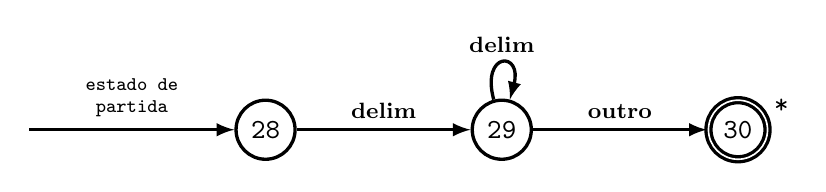
\begin{tikzpicture} 
            \coordinate (X) at (0, 6);

            \node[draw,circle,very thick] (A28) at (3, 6) { \texttt{28} };
            \node[draw,circle,very thick] (A29) at (6, 6) { \texttt{29} };
            \node[draw,circle,double,very thick] (A30) at (9, 6) { \texttt{30} };
           
            \node at (9.55, 6.3) { \texttt{*} };

%            \node[anchor=west] at (9.75, 6) { \footnotesize \texttt{retorne \{ \texttt{NUM}, $valor$\ \} } };

            \draw[very thick,-latex] (X) to node[above] { \scriptsize \texttt{\begin{tabular}{c}estado de\\ partida\end{tabular}} } (A28);
            \draw[very thick,-latex] (A28) to node[above] { \footnotesize $\mathbf{delim}$ } (A29);
            \draw[very thick,-latex] (A29) to [loop above] node[above] { \footnotesize $\mathbf{delim}$ } (A29);
            \draw[very thick,-latex] (A29) to node[above] { \footnotesize $\mathbf{outro}$ } (A30);

        \end{tikzpicture} 
    \end{figure}

\end{frame}

\begin{frame}[fragile]{Implementação dos digramas de transição em C++}
    \inputsnippet{cpp}{1}{19}{codes/diagramas.cpp}
\end{frame}

\begin{frame}[fragile]{Implementação dos digramas de transição em C++}
    \inputsnippet{cpp}{21}{35}{codes/diagramas.cpp}
\end{frame}

\begin{frame}[fragile]{Implementação dos digramas de transição em C++}
    \inputsnippet{cpp}{37}{46}{codes/diagramas.cpp}
\end{frame}

\begin{frame}[fragile]{Implementação dos digramas de transição em C++}
    \inputsnippet{cpp}{48}{62}{codes/diagramas.cpp}
\end{frame}

\begin{frame}[fragile]{Implementação dos digramas de transição em C++}
    \inputsnippet{cpp}{64}{83}{codes/diagramas.cpp}
\end{frame}

\begin{frame}[fragile]{Implementação dos digramas de transição em C++}
    \inputsnippet{cpp}{85}{92}{codes/diagramas.cpp}
\end{frame}

\begin{frame}[fragile]{Implementação dos digramas de transição em C++}
    \inputsnippet{cpp}{94}{112}{codes/diagramas.cpp}
\end{frame}

\begin{frame}[fragile]{Implementação dos digramas de transição em C++}
    \inputsnippet{cpp}{114}{126}{codes/diagramas.cpp}
\end{frame}

\begin{frame}[fragile]{Implementação dos digramas de transição em C++}
    \inputsnippet{cpp}{128}{142}{codes/diagramas.cpp}
\end{frame}
